% http://www.r-bloggers.com/time-series-plots-in-r/
% http://www.fromthebottomoftheheap.net/2013/10/23/time-series-plots-with-lattice-and-ggplot/


% ------------------------------------------------------------
% ------------------------------------------------------------

%%%%%%%%%%%%%%%%%%%%%%%%%%%%%%%%%%%%%

% Section: Plots of TS in R 

\section[Time Series Plots]{Time Series Plots}
%%%%%%%%%%%%%%%%%%%%%%%%%%%%%%%%%%%%%

%\subsection{Univariate Plots}
%%%%%%%%%%%%%%%%%%%%%%%%%%%%%%%%%%%%%%

%\begin{frame}[fragile]
% \frametitle{Univariate Time Series Plot  \footnote{This section is from the SCC Mini-Course "Introductory Time Series \\ with R" by Irina Kukuyeva}}

%To plot one variables one at a time, use \ttfamily plot(): \normalfont 
%    \begin{columns}
%      \column{0.55\textwidth}
%		\begin{lstlisting}
%data(EuStockMarkets)
%dax<-EuStockMarkets[, 1]
%plot(dax)
%		\end{lstlisting}

%      \column{0.45\textwidth}
%       \begin{center}
%         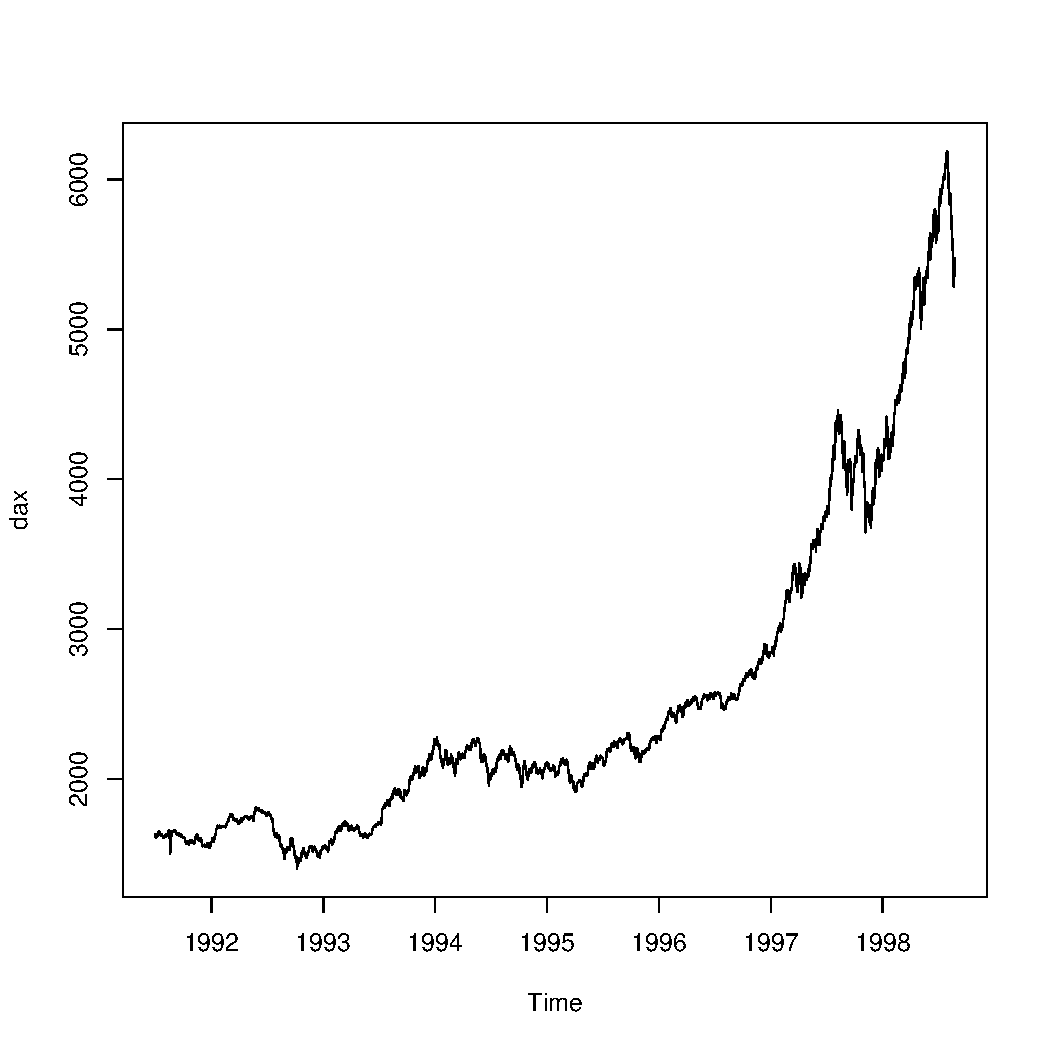
\includegraphics[width=0.95\textwidth]{images/daxPlot.pdf}
%        \end{center}
%      \end{columns}

%\end{frame}

%%%%%%% New frame
%\begin{frame}[allowframebreaks, fragile]
% \frametitle{Customizing the plot}

%To plot more than variables one at a time, use \ttfamily xyplot(): \normalfont
%		\begin{lstlisting}
%# After processing data as in Approach 1
%# load both libraries:
%library(lattice)
%library(zoo)
%data(EuStockMarkets)
%z<-EuStockMarkets
%xyplot(z, screen = c(1,1,1,1), col = 1:4, strip = FALSE)
%legend(1992, 5000, colnames(z), lty = 1, col = 1:4)
%		\end{lstlisting}

%       \begin{center}
%         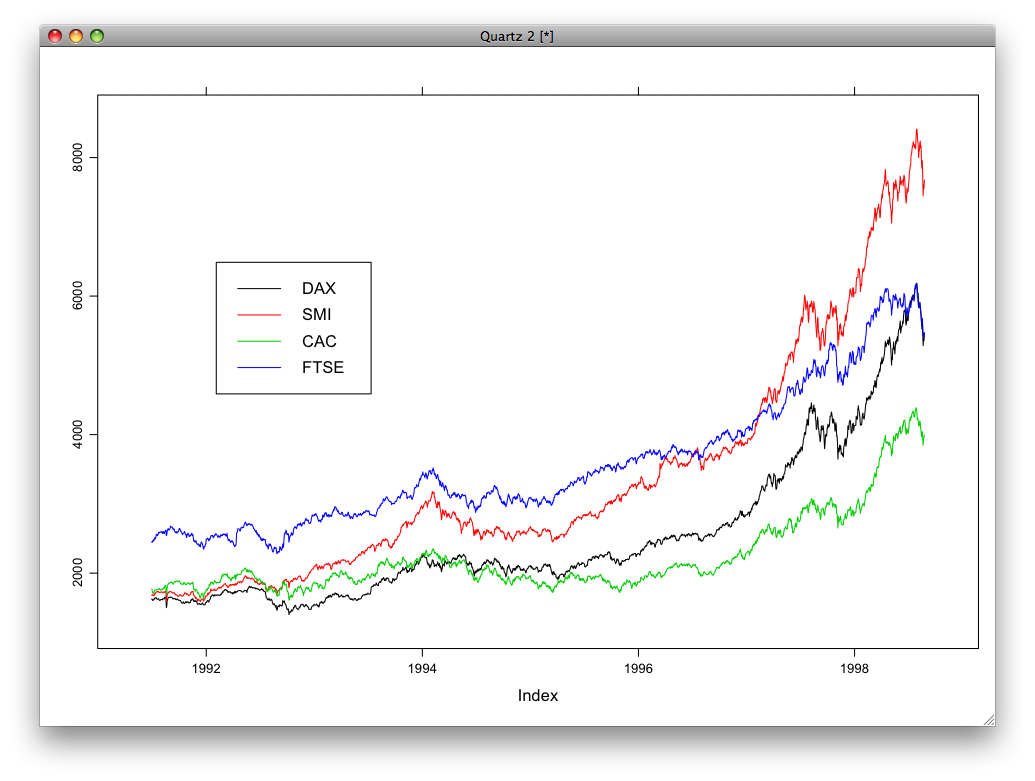
\includegraphics[width=0.85\textwidth]{images/stockPlot2}
%        \end{center}
%\end{frame}

%%%%%%%%%%%%%%%%%%%%%%%%%%%%%%%%%%%%%

\subsection{Multivariate Plots: Approach 1}

%%%%%%%%%%%%%%%%%%%%%%%%%%%%%%%%%%%%%

\begin{frame}[allowframebreaks, fragile]
 \frametitle{Multivariate Time Series Plots}
 \framesubtitle{Approach 1}

To plot more than variables one at a time, use \ttfamily mvtsplot()\normalfont [5]:
%\begin{itemize}
%	\item For documentation, go to: www.jstatsoft.org/v25/c01/paper 
%	\item Go to: http://www.biostat.jhsph.edu/$\sim$rpeng/RR/mvtsplot/
%	\item Copy the relevant R Code and paste it into the R Console. Press ENTER.
%	\item Plot your data
% \end{itemize}
		\begin{lstlisting}
library(mvtsplot)		
# Data = Daily Closing of Stock Indices:
data(EuStockMarkets)
# Purple=low, grey=medium, 
# green=high, white=missing values:
mvtsplot(EuStockMarkets)
		\end{lstlisting}

       \begin{center}
         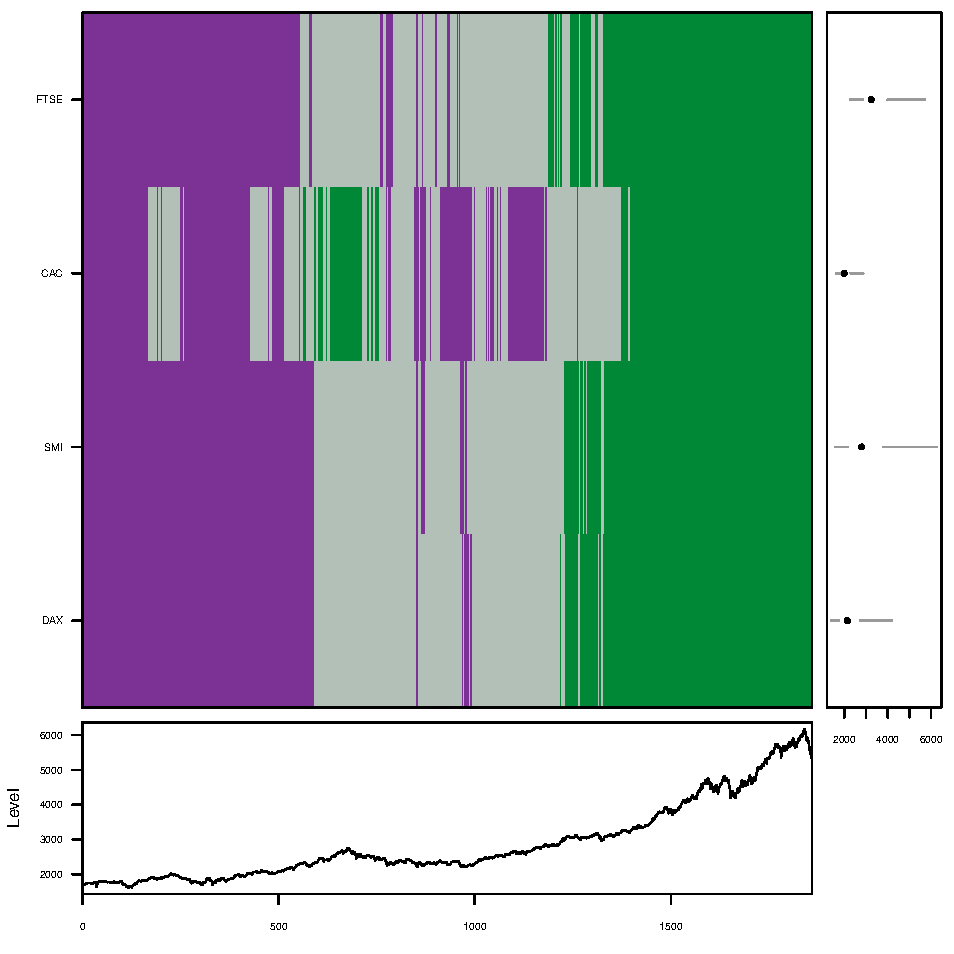
\includegraphics[width=0.6\textwidth]{images/Mtvsplot1.pdf}
        \end{center}

\end{frame}

\subsection{Multivariate Plots: Approach 2}
\begin{frame}[fragile, allowframebreaks]
 \frametitle{Multivariate Time Series Plots}
 \framesubtitle{Approach 2 (v0.2)}

Another way to plot more than one variable at a time, is via \ttfamily xyplot()\normalfont :

    \begin{lstlisting}
library(lattice) 
data(EuStockMarkets)
xyplot(EuStockMarkets)
   \end{lstlisting}


       \begin{center}
         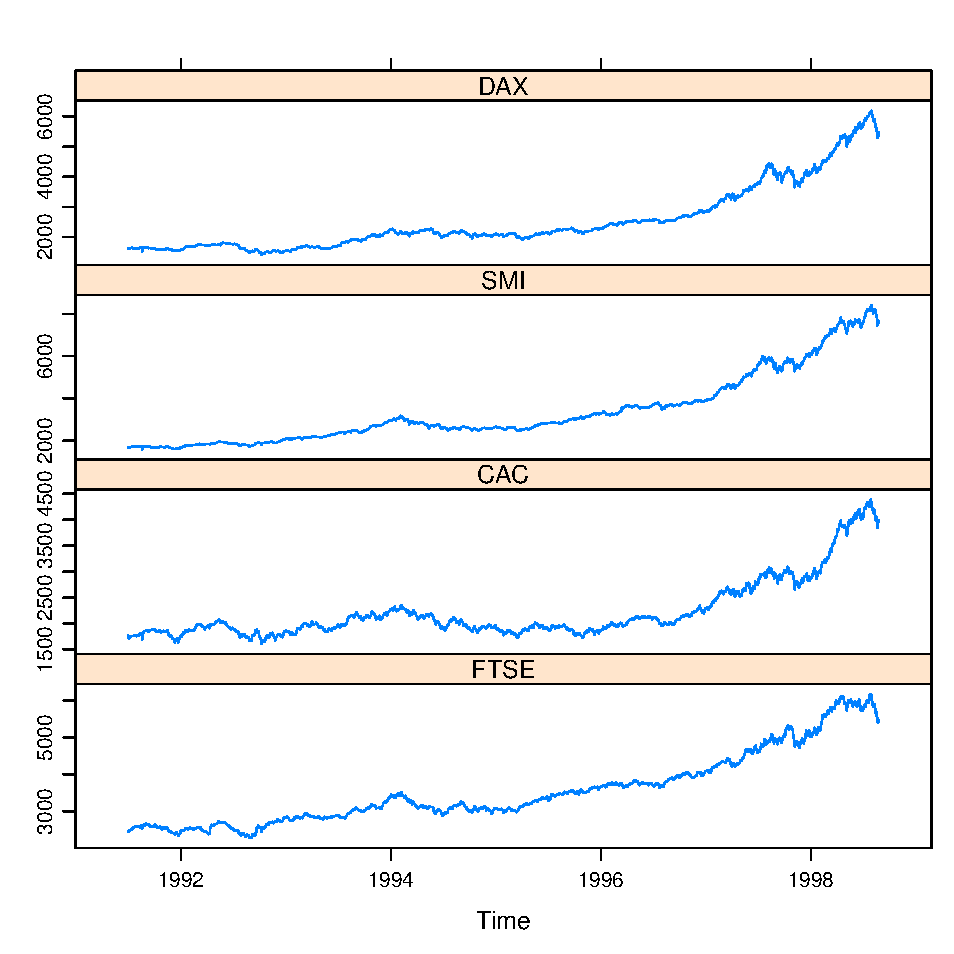
\includegraphics[width=0.6\textwidth]{images/stockPlot0.pdf}
        \end{center}
\end{frame}

\begin{frame}[fragile, allowframebreaks]
 \frametitle{Multivariate Time Series Plots}
 \framesubtitle{Approach 2 (v0.2)}

To customize the output, modify controls of \ttfamily xyplot()\normalfont :

    \begin{lstlisting}[ basicstyle=\small]
library(lattice)
library(reshape2)   
data(EuStockMarkets)
# Stack data per [2]:
df = cbind.data.frame(
  "id"=1:nrow(EuStockMarkets),
  EuStockMarkets
  )
df_stacked = melt(
  df,
  id="id"
  )
# Adding labels per [3]:
xyplot( df_stacked$value ~ df_stacked$id, 
  groups=df_stacked$variable,
  auto.key = list(space = "right"),
  scales = list(y = list(rot = 45),
                x = list(
                  at=c(0,500, 1000, 1500),
                  labels=seq(from=1992, to=1998, by=2)
                  )
                ),
  xlab="Time",
  ylab="Value"
  )
    \end{lstlisting}
%% To modify legend's tick marks
%% per http://grokbase.com/t/r/r-help/073mmn16mn/r-lattice-key-legend-with-both-points-and-lines
%%
% xyplot(1:10 ~ 1:10,
%   key = list(
%     text = list(c("prices", "means")),
%     lines = list(
%     pch = c("*", ""), type = c("p", "l"),
%     cex = 2, col = "red", lwd = 3)
%     )
% )
       \begin{center}
         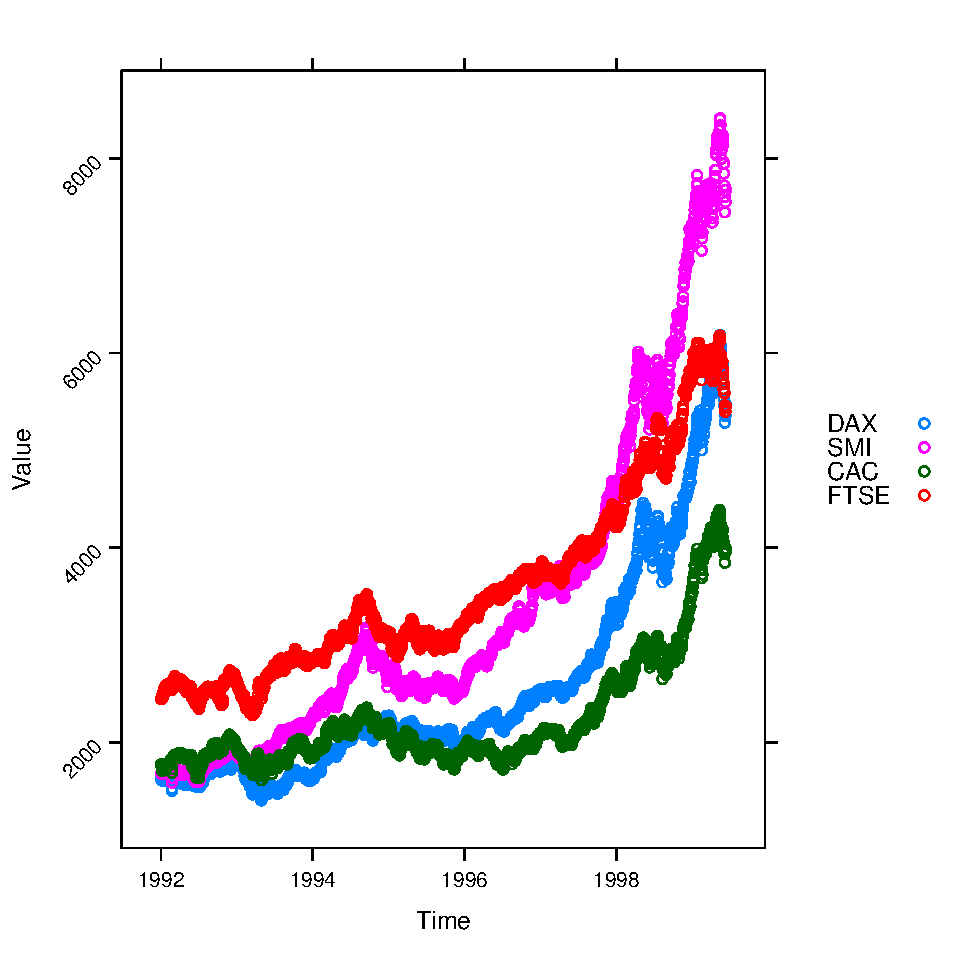
\includegraphics[width=0.6\textwidth]{images/stockPlot1.pdf}
        \end{center}
\end{frame}

%%%%%% New frame
\subsection{Multivariate Plots: Approach 3}
\begin{frame}[allowframebreaks, fragile]
 \frametitle{Multivariate Time Series Plots}
 \framesubtitle{Approach 3}

Another way to plot more than one variable at a time, is via \ttfamily ggplot()\normalfont :
		\begin{lstlisting}
library(ggplot2)
library(reshape2)   
data(EuStockMarkets)
df = cbind.data.frame(
  "id"=1:nrow(EuStockMarkets),
  EuStockMarkets
  )
df_stacked = melt(
  df,
  id="id"
  )
# Ading labels per [4]:
ggplot(
  data = df_stacked,
  aes(x = id, y = value, color = variable)
  ) +
  geom_point() +
  scale_x_discrete(name="Time",
    breaks=seq(from=0, to=1500, by=500),
    labels=seq(from=1992, to=1998, by=2)
    )
		\end{lstlisting}

       \begin{center}
         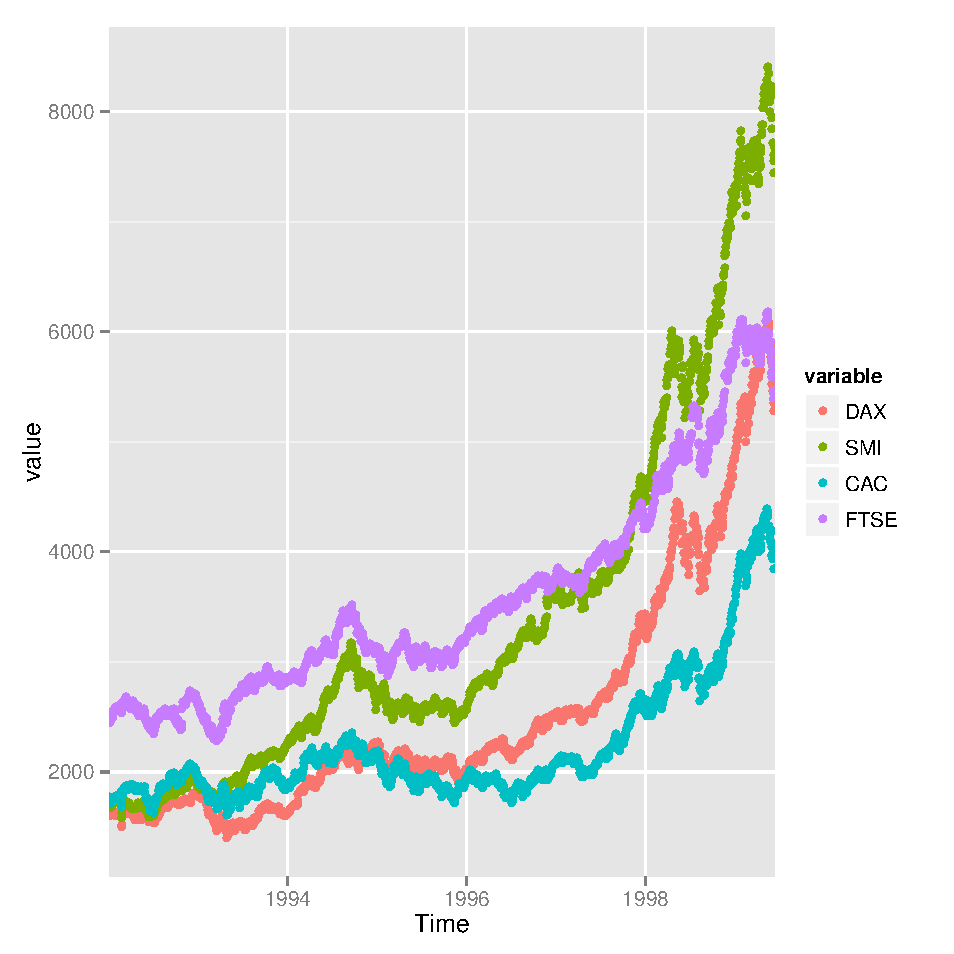
\includegraphics[scale=0.4]{images/stockPlot2.pdf}
        \end{center}
\end{frame}
%
%%___________________________________
%\subsection{Customizing Plots}
%%___________________________________

%\begin{frame}[allowframebreaks, fragile]
% \frametitle{Customizing Plots}

%%
%%To plot more than variables one at a time, use \ttfamily xyplot(): \normalfont
%%		\begin{lstlisting}

%%		\end{lstlisting}

%%       \begin{center}
%%         \includegraphics[width=0.85\textwidth]{images/???}
%%        \end{center}
%\end{frame}

% % ------------------------------------------------------------
% % ------------------------------------------------------------
\subsection{Exercise II}
\begin{frame}[fragile]
	\frametitle{Exercise II}
	Analyze the approval ratings of the President of the United States in the data set\ttfamily presidents. \normalfont  What stands out and why?\\
  \vspace{10pt}
  \noindent Hints: \small
    \begin{itemize}
      \item Load the data set \ttfamily presidents.\normalfont
      \item Convert the data set to be in matrix format, one row per year.
%           \begin{lstlisting}[ basicstyle=\footnotesize]
% presidents_mat = matrix(
%   presidents, 
%   ncol=4, 
%   byrow=TRUE
%   )
%           \end{lstlisting}
      \item Plot the data set.
      \item Examine the result.
    \end{itemize}
    \normalsize
\end{frame}
